\documentclass[xcolor=table]{beamer}
\usepackage[table,xcdraw]{xcolor}
\usepackage[utf8]{inputenc}
\usepackage[utf8]{inputenc}
\usepackage{epigraph}
\usepackage{graphicx}
\usepackage[left=25mm,right=25mm,top=2cm,bottom=2cm]{geometry}
\usepackage{indentfirst}
\usepackage{hyperref}
\usepackage{amsmath}
\usepackage{xcolor}
\usepackage{float}
\usepackage{wrapfig}
\usepackage{subfig}
\usepackage{derivative}
\usepackage[table,xcdraw]{xcolor}
\usepackage[english, russian]{babel}
\usepackage{setspace}

\usetheme{Madrid}
\usecolortheme{default}

%------------------------------------------------------------
%This block of code defines the information to appear in the
%Title page
\title[Исследование свободных колебаний связанных маятников] %optional
{Исследование свободных колебаний связанных маятников}

%\subtitle{Начало}

\author[Аношин, Масов] 
{М.~Аношин\inst{1} \and Е. ~Масов\inst{1}}

\date[15.10.2022] 
{МФТИ, Октябрь 2022}

\begin{document}
\frame{\titlepage}

\section{Цель работы}
\begin{frame}\frametitle{Цель работы}
    \begin{itemize}
        \item Изучение колебательной системы с двумя степенями свободы
    \end{itemize}
    \vspace{15}
    \large{\textbf{В работе используются:}}\\
    \begin{itemize}
        \large \normalsize{Установка с двумя одинаковыми маятниками измерительная линейка, программа STAT}
    \end{itemize}
\end{frame}


\begin{frame}\frametitle{Установка}
    \begin{figure}
        \centering
        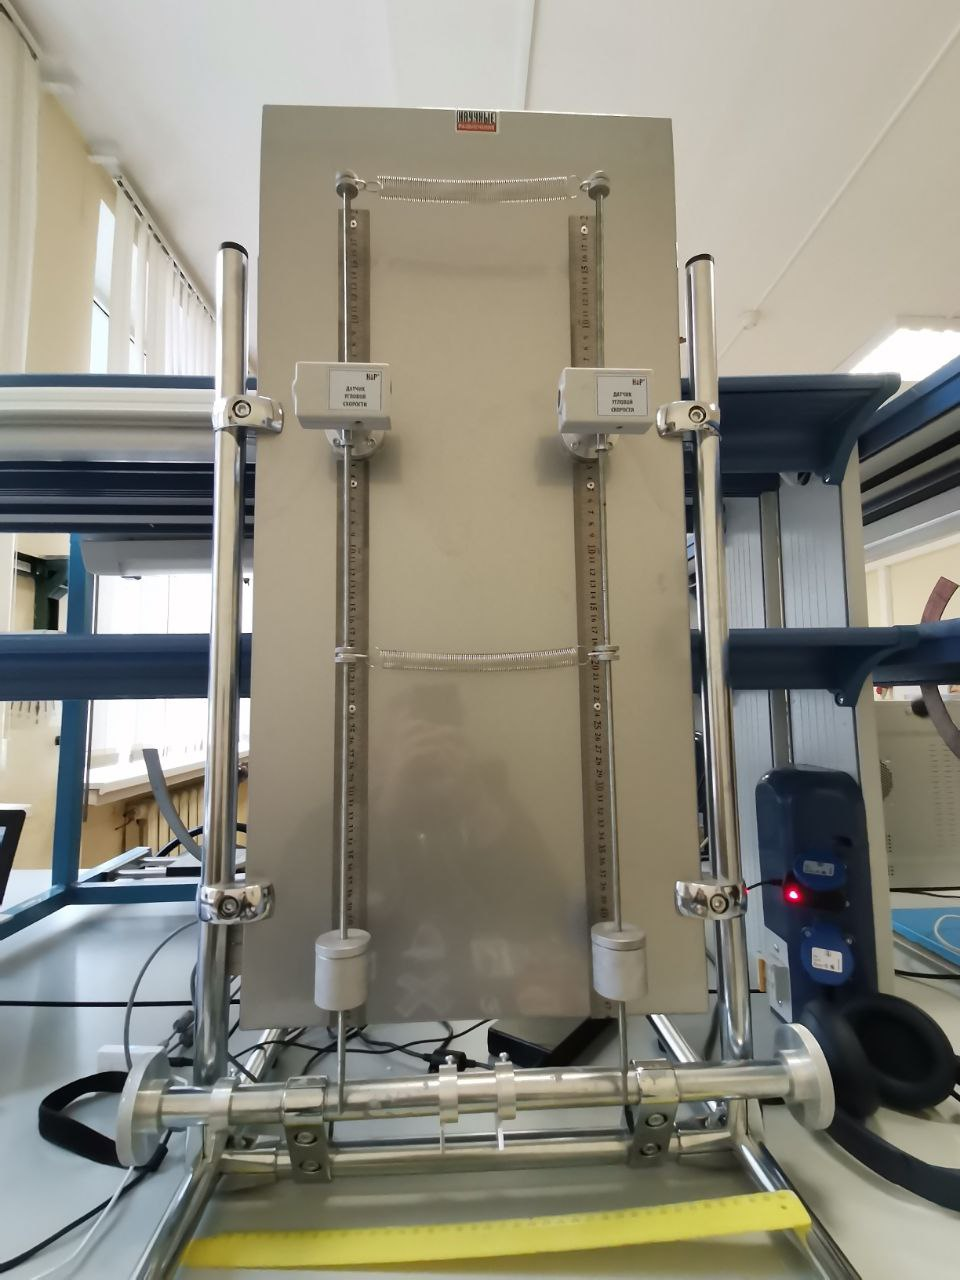
\includegraphics[scale=0.15]{installation.jpg}
        \caption{1. Полная фотография установки}
        \label{fig:my_label}
    \end{figure}
\end{frame}


\begin{frame}\frametitle{Теория}
    $$ML^2 \ddot{\phi} = - MgL \sin{\phi} + Fd\cos{\phi}, \;\;\; \phi << 1$$
    $$ML^2 \ddot{\phi} = - MgL \phi + Fd$$
    $$ML^2 \ddot{\phi} + MgL \phi - kLd (\phi_2 - \phi_1) = 0$$
    $$\ddot{\phi_1} + \frac{g}{L} \phi_1 - \frac{kd}{ML} (\phi_2 - \phi_1) = 0$$
    $$\ddot{\phi_2} + \frac{g}{L} \phi_2 - \frac{kd}{ML} (\phi_1 - \phi_2) = 0$$
    $$\phi(t) = A\cos{(\omega_1 t + \alpha)} + B\cos{(\omega_2 t + \beta)}$$
    \centering
    где $\omega_1 = \sqrt{\frac{g}{L}}, \;\; \omega_2 = \sqrt{\frac{g}{L} + \frac{2kd}{ML}}, \;\;\; k << \frac{Mg}{L}$
    $$\omega_2 \approx \sqrt{\frac{g}{L}} + \frac{kd}{ML} = \omega_1 + \frac{kd}{ML}$$
\end{frame}


\begin{frame}{Результаты измерений}
    \begin{figure}
        \centering
        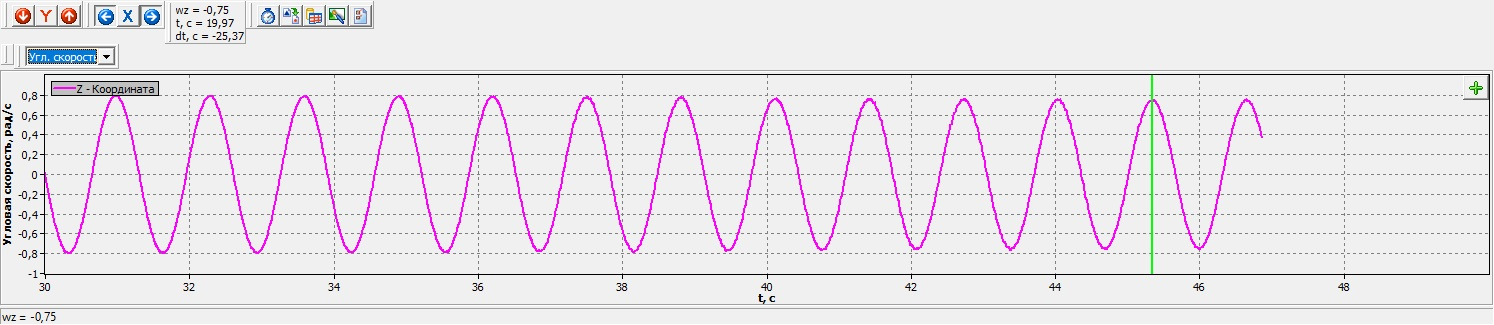
\includegraphics[scale = 0.8]{images/Oscillation period.jpg}
        \caption{Рис.2 График свободных колебаний}
        \label{fig:my_label}
    \end{figure}
\end{frame}


\begin{frame}{Результаты измерений}
    \begin{figure}[h]
        \centering
        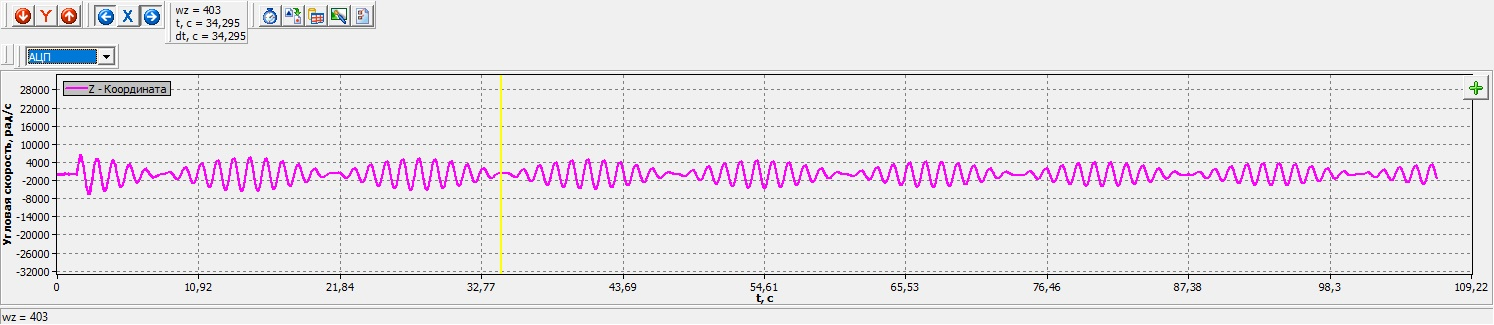
\includegraphics[scale = 0.6]{images/beats.jpg}
        \caption{3. Биения}
        \label{}
    \end{figure}
\end{frame}


\begin{frame}{Результаты измерений}
    \begin{figure}[h]
        \centering
        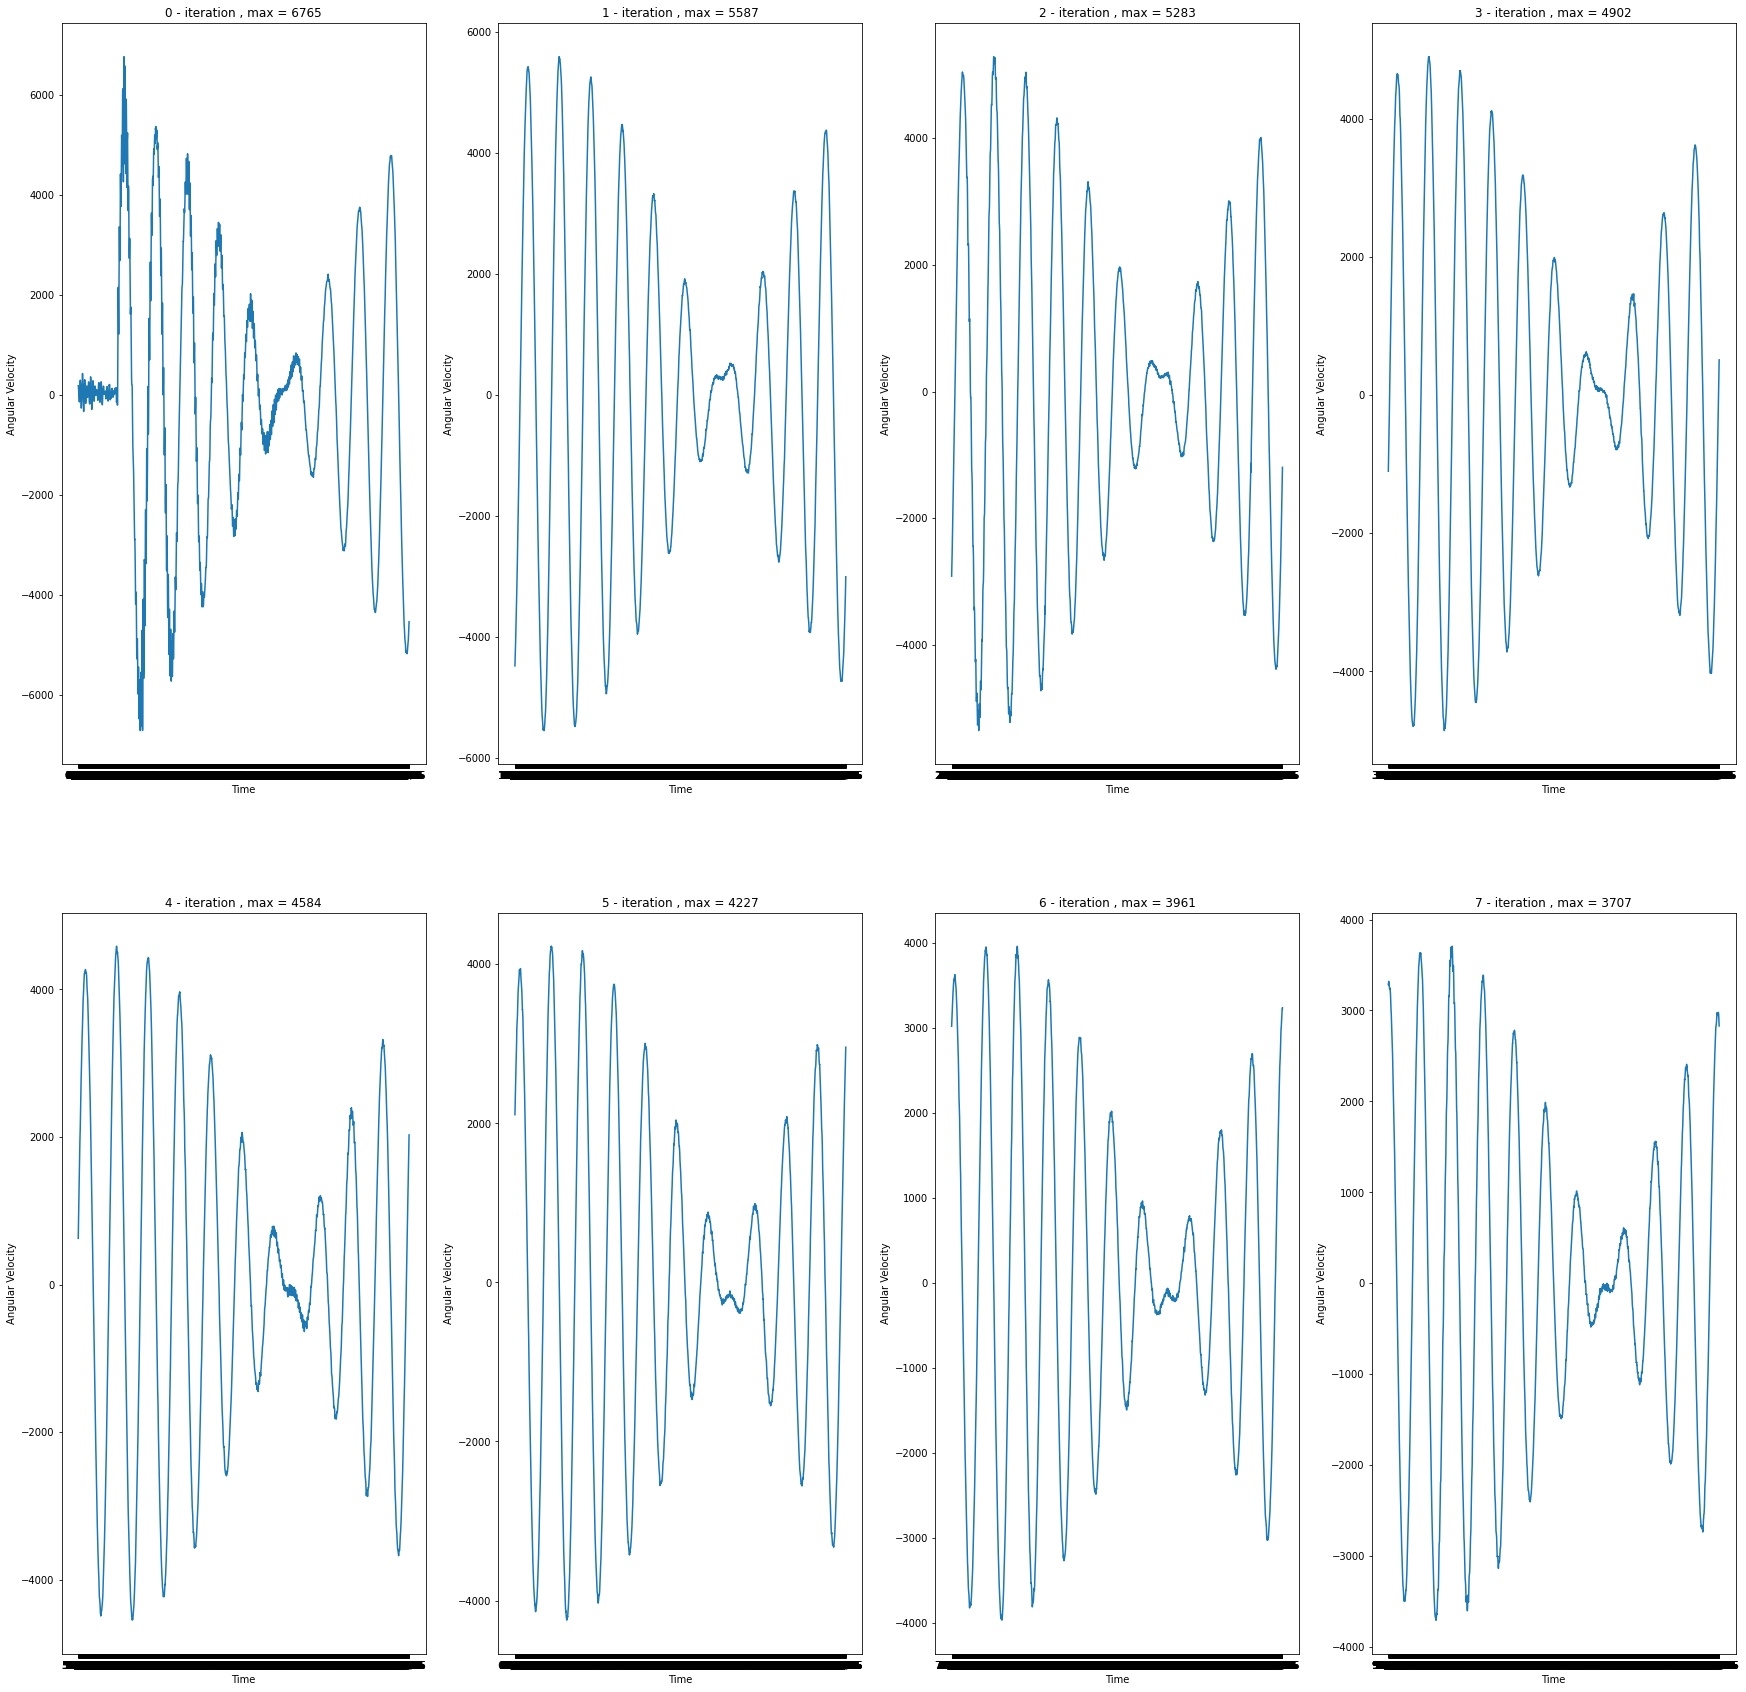
\includegraphics[scale = 0.12]{Oscillation_groups.jpg}
        \caption{4. }
        \label{}
    \end{figure}
\end{frame}


\begin{frame}{Результаты измерений}
    $$L = 40 cm, \;\; d = 20 cm \;\; x_0 = 8.5 cm$$
    $$\phi_0 = arctg\frac{x_0}{L + h_0} = 12^{\circ} \;\;\;, h_0 = 10 cm$$
    \begin{table}[h]
        \centering
        \begin{tabular}{|c|c|c|}
             \hline
             Колебания & T, s & N \\
             \hline
             Свободные & 1,3 \pm 0.01 & 0 \\
             Синфазные & 1,31 \pm 0.01 & 2 \\
             Синфазные & 1,29 \pm 0.01 & 1 \\
             Антифазные & 1,21 \pm 0.01 & 2 \\
             Антифазные & 1,24 \pm 0.01 & 1 \\
             Биения & 13,26 \pm 0.01 & 2 \\
             Биения & 24,4 \pm 0.01 & 1 \\
             \hline
        \end{tabular}
        \caption{Результаты измерений}
        \label{tab:my_label}
    \end{table}
\end{frame}


\begin{frame}{Результаты измерений. Декремент затухания}
    \begin{figure}[h]
        \centering
        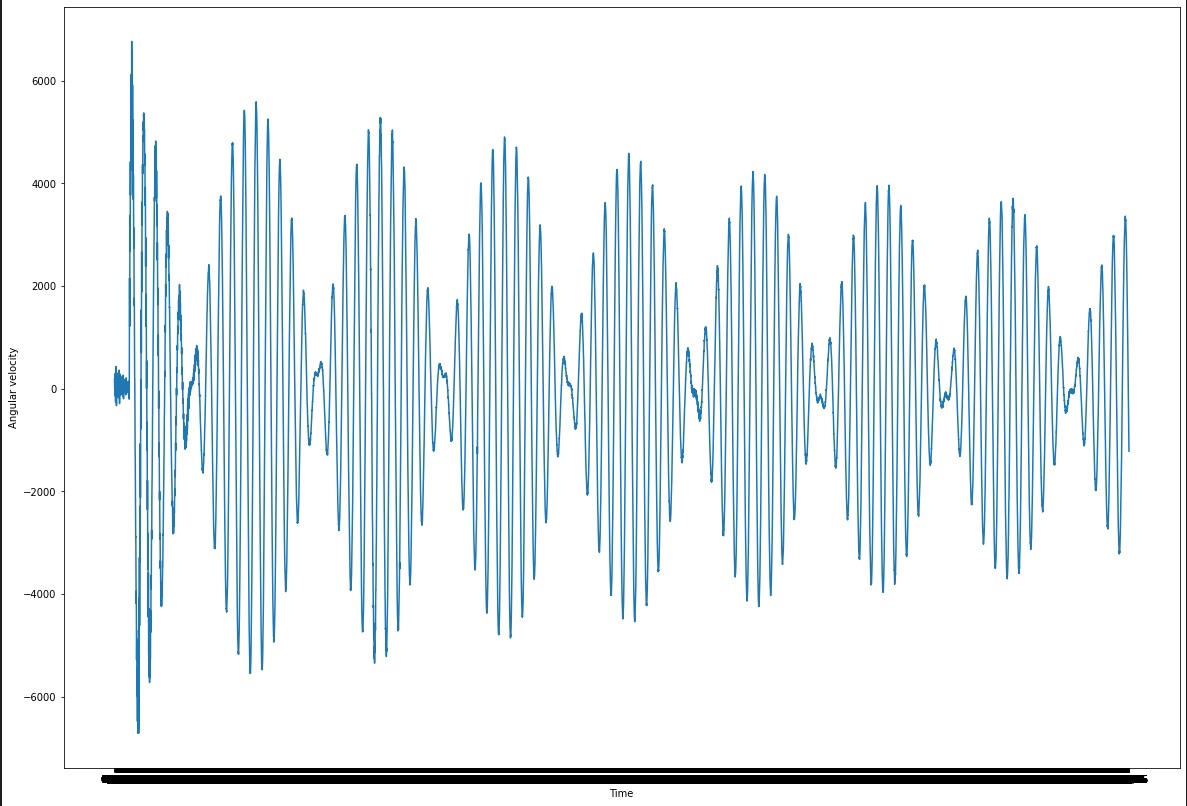
\includegraphics[scale = 0.25]{Oscillation.jpg}
        \caption{5. }
        \label{}
    \end{figure}
\end{frame}


\begin{frame}{Результаты измерений. Декремент затухания}
    \begin{figure}[h]
        \centering
        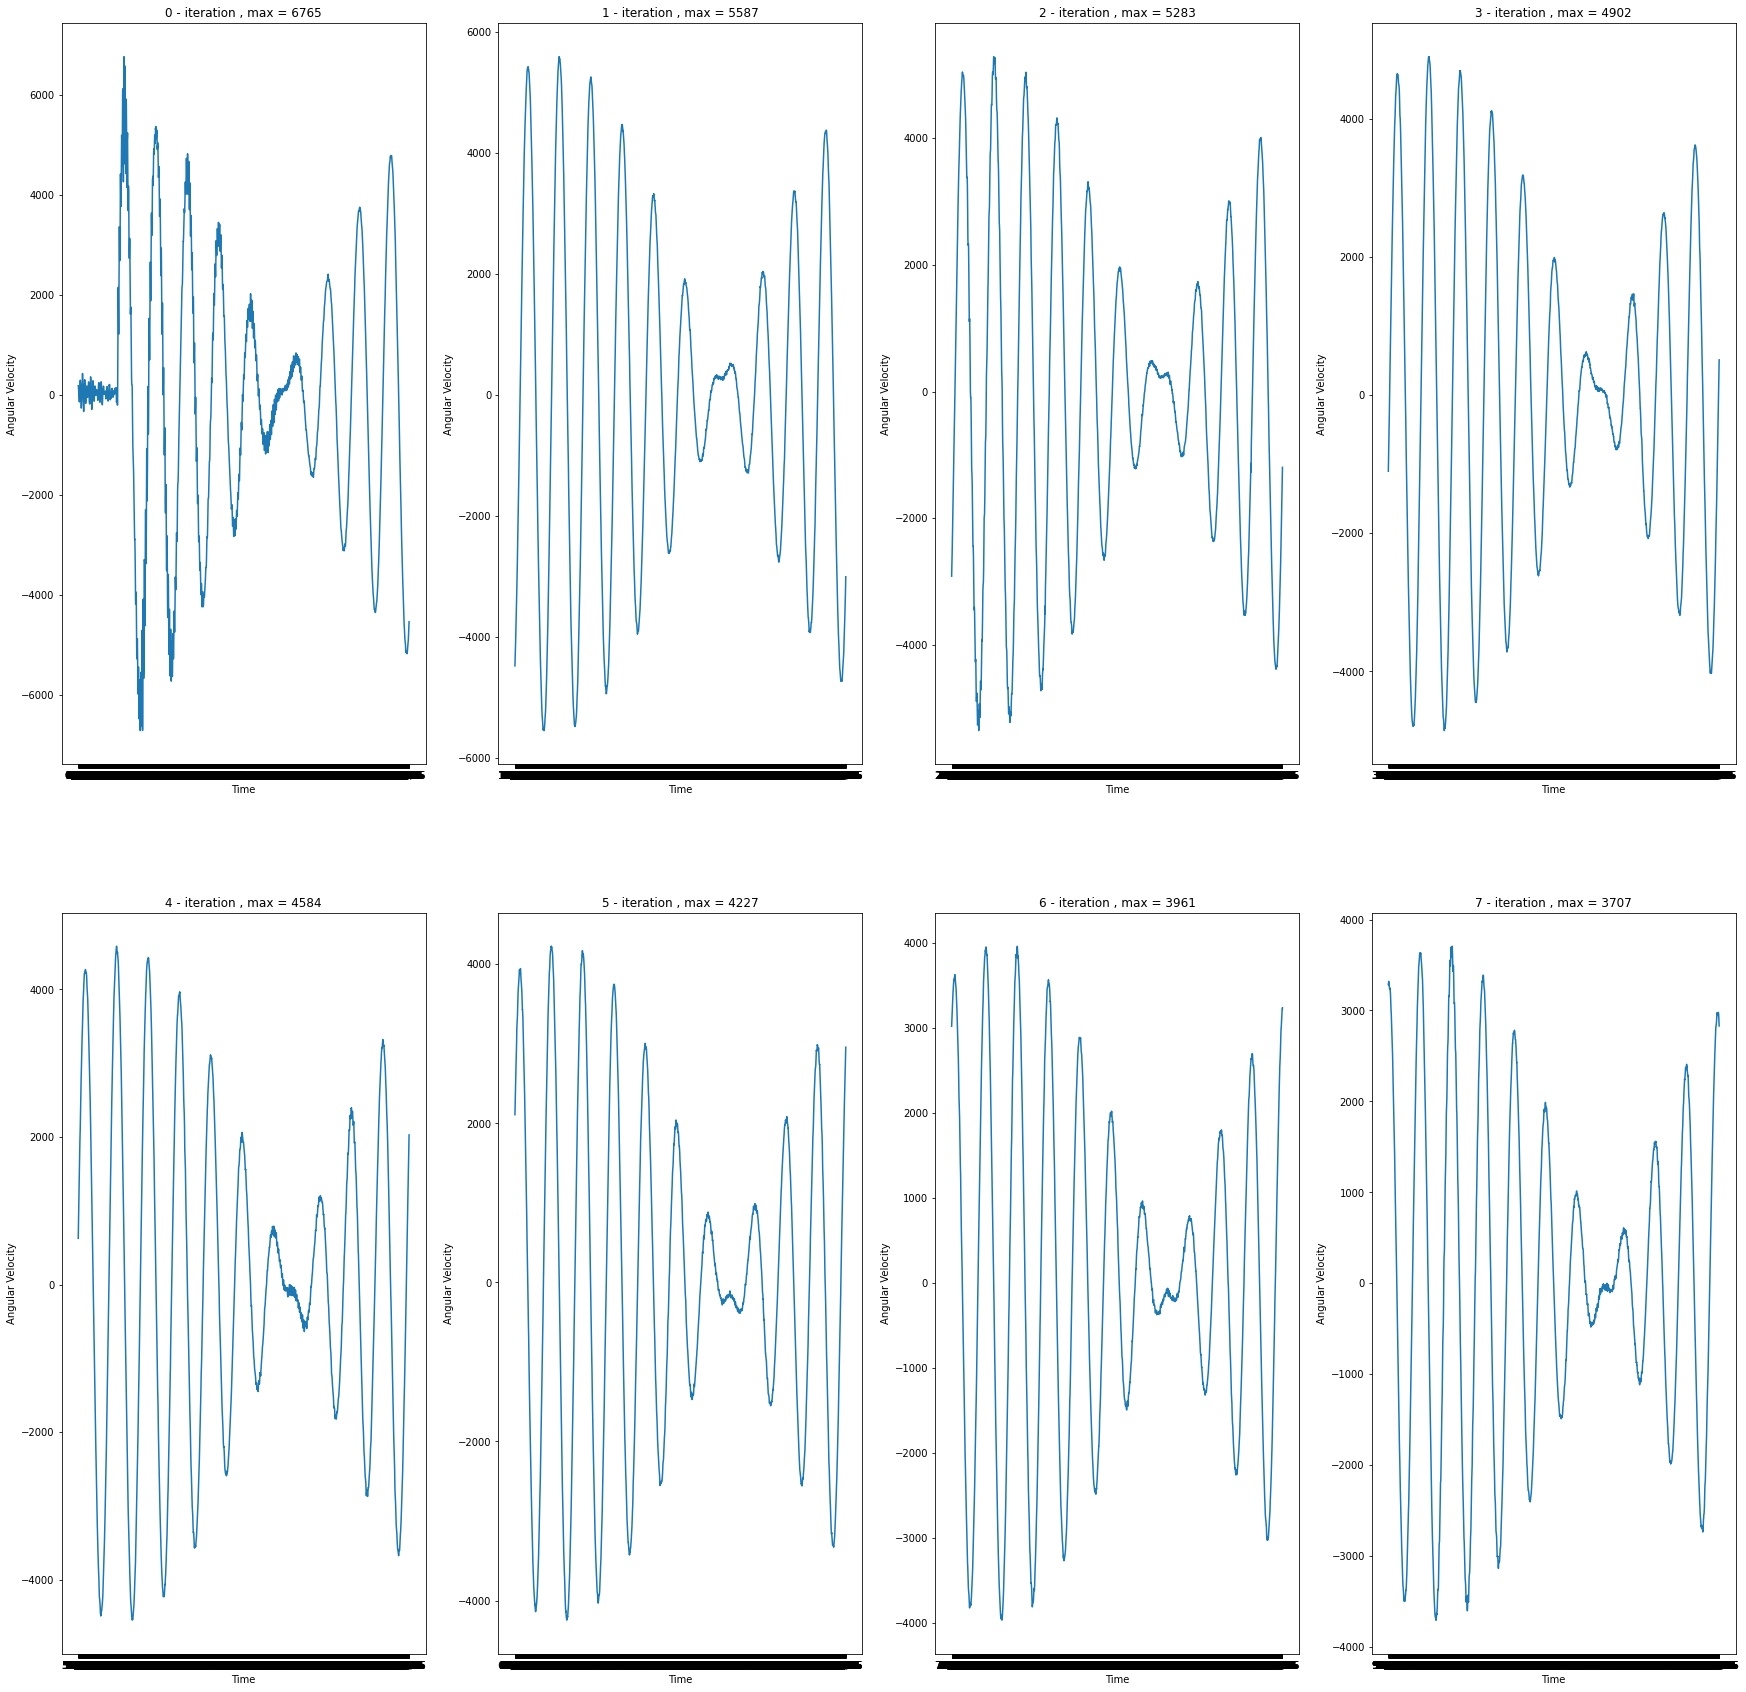
\includegraphics[scale = 0.12]{Oscillation_groups.jpg}
        \caption{6. }
        \label{}
    \end{figure}
\end{frame}


\begin{frame}{Результаты измерений. Декремент затухания}
    \begin{figure}[h]
        \centering
        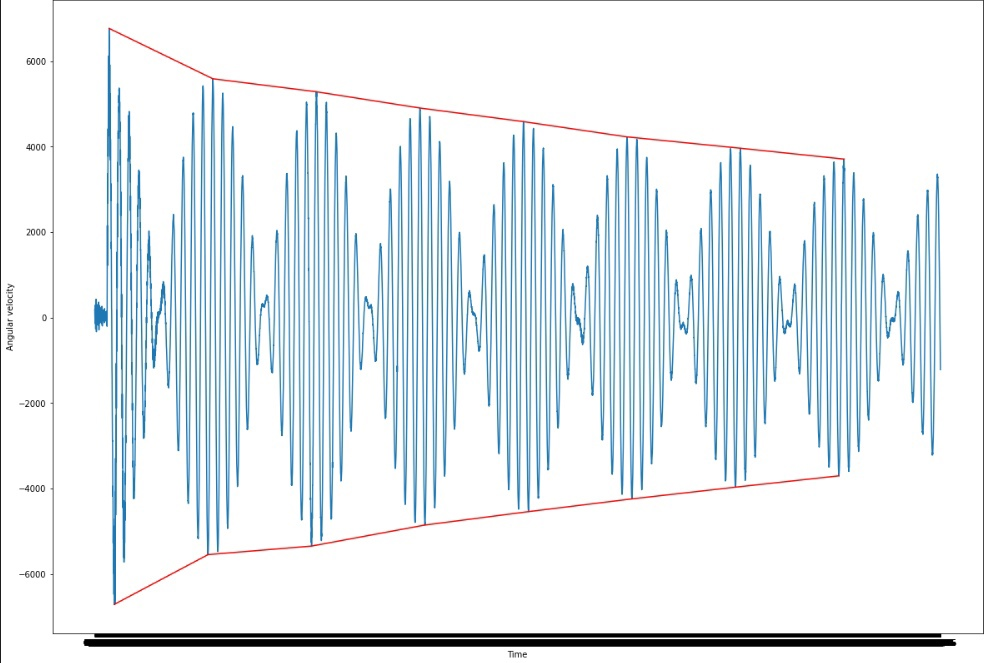
\includegraphics[scale = 0.28]{decrement.jpg}
        \caption{7. }
        \label{}
    \end{figure}
\end{frame}

\begin{frame}{Результаты измерений. Декремент затухания}
    \begin{figure}
            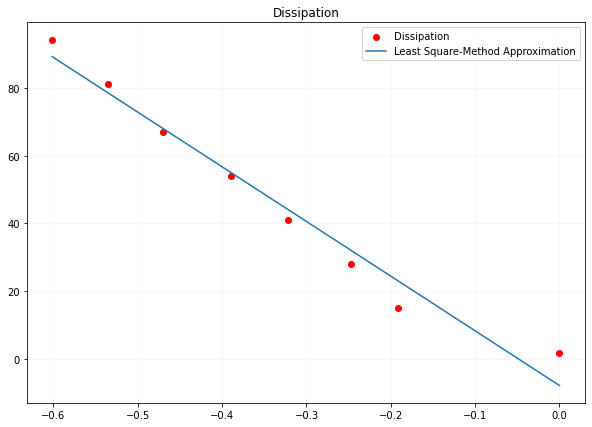
\includegraphics[width=0.9\linewidth]{images/Diss.png}
            \caption{8. }
            \label{fig:4}
    \end{figure}
\end{frame}

\begin{frame}{Результаты измерений. Декремент затухания}
    \centering
    \begin{figure}
        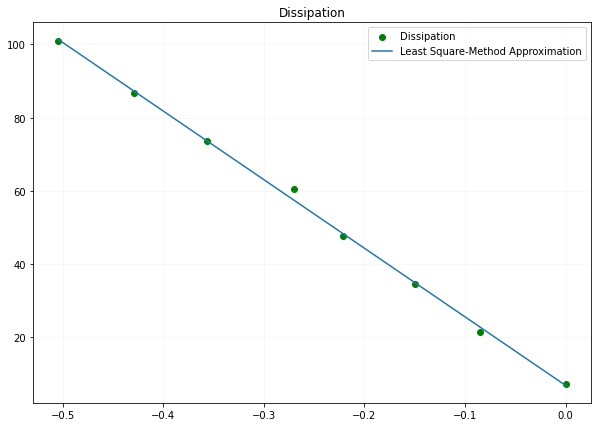
\includegraphics[width=0.9\linewidth]{images/Diss2.png}
        \caption{9. }
        \label{fig:5}
    \end{figure}
\end{frame}

\begin{frame}{Результаты измерений. Декремент затухания}
    $$\phi(t) = (A\cos{(\omega_1 t + \alpha)} + B\cos{(\omega_2 t + \beta)) \cdot e^{-\beta t}}$$
    $$\lambda = \beta T = \frac{\phi_n}{\phi_{n+1}}$$
    $$\beta = 0.057 \pm 0.005$$$
\end{frame}

\end{document}